\section{Worlds beyond Earth's range}

An Earth value in a model holds where a world's governing ratios equal Earth's, and its error grows with the
world's distance from them. Four ratios govern most of the values found in these models
(Table~\ref{tab:regime}): the scale height over the radius, which fixes the geometry of the sunlit and
radiating air; the mass of air over each square metre, which fixes the absorber paths that broadband
radiation fits were made on and the pressures that radiation tables span; the gravity, which fixes the
height of each pressure level and the fall of every particle; and the solar day, which fixes whatever a
formula counts per day. Found and constructed worlds lie off Earth's values in different directions
(Figure~\ref{fig:regimes}). Titan's air holds ten times Earth's mass over each square metre and Venus's a
hundred times, and their solar days of 16 and 117 Earth days place both far along the day axis; present Mars
departs mainly in its thin column, and Earth-like planets that rotate slowly depart along the day axis
alone. The breathable Moon departs along all four at once, in air close to Earth's.\claim{W02}

\begin{figure}[tbp]
\centering
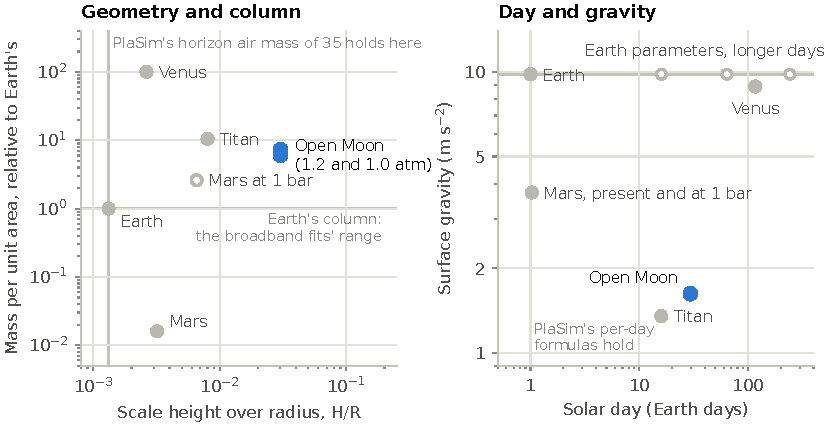
\includegraphics[width=\textwidth]{figures/fig_regimes.pdf}
\caption{Found and constructed worlds against the ratios on which the models' Earth assumptions depend.
Left: scale height over radius against the air's mass per unit area, relative to Earth's; PlaSim's horizon
air mass is exact on the vertical line through Earth, and its broadband radiation fits were made near the
horizontal one. Right: solar day against surface gravity; PlaSim's per-day formulas are exact on the
vertical line, and released CM1 holds only where the two lines cross. Grey filled points are found worlds;
open points are constructed or illustrative ones (Mars held at 1~bar; Earth-like planets with solar days of
16, 64 and 243 days); blue points are the breathable Moon at 1.2 and 1.0~atm. Scale heights use each world's
surface temperature and mean molar mass.}
\label{fig:regimes}
\end{figure}

The models take the case's scenario as fixed conditions. The TSIS-1 solar spectrum
\autocite{coddington2021tsis}, passed through a titania shield in space, brings 1,235~W\,m$^{-2}$ to the top
of the air, dimmed evenly at every wavelength to 1,198~W\,m$^{-2}$ in the design case, a scale of 0.970
chosen so that the GCM's global-mean surface settles at the design temperature of 295~K; a change in the
physics therefore appears as a change in the dimming the design needs. The shield removes the ultraviolet
that would make ozone, so the air holds none.\claim{S07}\claim{G04} Beneath the shield the air holds
121,590~Pa at the water level, with oxygen at Earth's partial pressure of 21,227~Pa (17.5\% of the air),
argon in Earth's ratio to nitrogen, 400~ppm of carbon dioxide and nitrogen for the balance; because the land
stands above the water level, the surface pressure averages 1.16~atm over the globe and ranges from 1.02 to
1.22~atm.\claim{S05} At the ground, seas fill the lunar basins to 28\% of the surface and rain-fed lakes
stand at their own levels, so that 759 of the GCM's 2,048 cells, 40\% of its surface, hold
water;\claim{S06} the seas are a 50~m slab with sea ice, and the land has a placeholder albedo of 0.2.

\begin{table}[t]
\caption{The ratios that separate the breathable Moon from Earth, and the model parts that depend on each.
Lunar values are for the 1.2~atm design case; scale heights use the surface temperature and the air's mean
molar mass; horizon air masses are Chapman's grazing factor $\sqrt{\pi R/2H}$ for an isothermal air, which
PlaSim's code sets at 35 for Earth. Rows marked $^\dagger$ are CM1 results for the case, conditional model
results; the grid for deep convection is a nominal scale from the dry dynamics' similarity; the other lunar
values are scenario inputs or calculations from them.}
\label{tab:regime}
\small
\begin{tabularx}{\textwidth}{@{}lrrL@{}}
\toprule
Quantity & Earth & Moon & Model parts that depend on it \\
\midrule
Surface gravity (m\,s$^{-2}$) & 9.81 & 1.62 & Dynamics; fall speeds; sea roughness; wave dispersion; heights in pressure terms \\
Surface pressure at the water level (bar) & 1.01 & 1.22 & RRTMG's tables, whose highest pressure is 1.05~bar \\
Air over each square metre (t) & 10.3 & 74.9 & Broadband absorber paths fitted on Earth's \\
Scale height at the surface (km) & 8.4 & 52 & Every height-based formula \\
Scale height over radius & 0.0013 & 0.030 & Flat, sunlit-only columns; the thin shell \\
Horizon air mass of well-mixed air & 34.5 & 7.2 & Earth's slant factor, fixed in PlaSim \\
Solar day (Earth days) & 1 & 29.53 & Formulas written per day; the soil's thermal wave; the model calendar \\
Sidereal rotation (Earth days) & 0.997 & 27.32 & ExoPlaSim's Sun clock; the Coriolis parameter \\
Tilt of the equator (\textdegree) & 23.44 & 1.54 & ExoPlaSim's orbit default \\
Height of the 0\,\textdegree C level (km)$^\dagger$ & 4.5--5 & 25 & Ground-strike rules; the charging zone \\
Tops of deep storm cloud (km)$^\dagger$ & 15--18 & 55--80 & Model tops; the levels of cold cloud \\
Fall speed of rain, relative & 1 & 0.34 & Evaporation of falling rain \\
Grid for deep convection (km) & 1 & 6 & Cost; the meaning of a resolution \\
\bottomrule
\end{tabularx}
\end{table}

Every path through the case's air is longer than its counterpart on Earth (Table~\ref{tab:regime}). With
7.25 times Earth's mass over each square metre, the design case's GCM column holds 170~kg\,m$^{-2}$ of
water vapour, and 348~kg\,m$^{-2}$ in its warmest test, where Earth's holds about 25
\autocite{trenberth2005trends}.\claim{S08} A scale height of about 52~km against a radius of 1,737~km places
the air's mass on average 48.6~km above the ground, where a shell has 5.8\% more area than the ground
beneath it, and straight rays through the design column give horizon air masses of 7.1 for well-mixed air
and 13.5 for water vapour, against the 35 of PlaSim's formula, written for Earth.\claim{S09} Sunlight
reaches far past each column's horizon: a full Earth day after sunset, about half the air above a place
still lies above the Moon's geometric shadow.\claim{S04} At these heights the thin-shell approximation of
the dynamics also becomes inexact. Gravity at the 86~km tropopause is 9\% below its surface value, a column
with gravity falling as $GM/r^2$ holds about 5\% more air per unit area than $p_s/g_s$, and spherical shells
with that gravity hold 11.5\% more over each square metre of ground than $p_s/g_s$.\claim{S10}

Gravity's surface value matters more. A sixth of Earth's gravity raises every pressure level sixfold in
height, so a formula written in metres places its features six times too low; it slows the fall of droplets
sixfold, of rain about threefold and of graupel 2.3-fold; it lengthens the roughness of a wind-driven sea
sixfold for the same friction velocity \autocite{charnock1955wind}; and it slows a deep-water wave of a
given length to 0.41 of its speed on Earth.\claim{S11} The dry dynamics stretch about sixfold in size and
duration at the same speeds, so a 6~km column of a cloud-resolving model stands for about 1~km at Earth's
scale, while the microphysics and the radiation keep their own scales; a pair of runs designed to measure how far
lunar convection departs from Earth's convection stretched sixfold failed to convect.\claim{S12} The 29.53-day solar day deepens the soil's thermal wave to about
0.6~m, $\sqrt{29.53}\approx5.4$ times the depth of Earth's diurnal wave, and multiplies nearly thirtyfold
whatever a formula counts per day; the 27.32-day rotation sets a Coriolis parameter of
\SI{5.2e-6}{s^{-1}} at 80\textdegree, an inertial period of 14 Earth days.\claim{S13} The tilt of
1.54\textdegree\ gives the poles a grazing Sun all year.
